\section*{Instrucciones:}

La tarea se entrega y se resuelve en equipos de máximo 3 integrantes (1 a 3 personas). La tarea se entrega virtualmente en formato pdf tanto si son fotos de cuaderno, está realizada en word, en LATEX, etc.

No habrán reposiciones de tareas. Las tareas se pueden entregar con máximo 2 días de retraso para
ser evaluadas sobre 8.

\textbf{Puntos Totales: 100}

\textbf{Tiempo estimado: $\approx$ 2hrs 10 min}

\section*{Ejercicios}

\begin{enumerate}
    \item Para cada uno de los siguientes enunciados identifica el tipo de propiedad e identifica:

    \begin{itemize}
        \item \textit{La cosa mala que nunca sucede en caso de que sea una propiedad segura.}

        \item \textit{La cosa buena que sucederá en caso de que sea una propiedad de viveza.}
    \end{itemize}

    \begin{enumerate}
        \item La inflación sube año con año
        
        \item Si Bob quiere entrar al patio a dejar comida eventualmente entrará
        
        \item Cada historia concurrente de esta implementación se puede transformar siempre a una implementación secuencial correcta
        
        \item El candado se liberará en algún momento

        \item El retraso de un proceso detendrá a otros eventualmente.

        \item El retraso de un proceso nunca detiene a otros.

    \end{enumerate}

    \hfill

    \item Muestra un ejemplo de una ejecución de la implementación de Filter en la que a un hilo A lo rebasa más de una vez cualquier hilo B considera un número n de hilos mayor a 10. Explica porque no se cumple la propiedad de Justicia. Hint: Puedes mostrar una imagen de una ejecución o describirla

    \hfill

    \item Argumenta si la siguiente implementación (VictimAround) de un candado para dos hilos cumple con

    \begin{enumerate}
        \item Exclusión mutua

        \item Deadlock-free

        \item Starvation-free
    \end{enumerate}
    
    
    \textit{Hint: Si no lo cumple, describe un ejemplo de una ejecución. Si lo cumple, encuentra la invariante y justifica el porqué}

    \begin{center}
            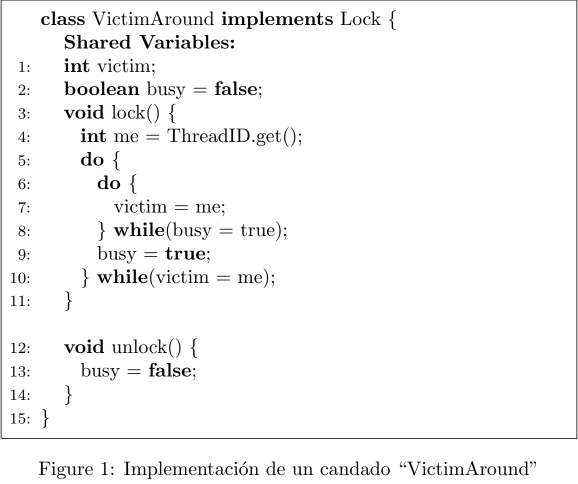
\includegraphics[width = 12 cm]{images/Figure1_tarea2.png}
    \end{center}

    \hfill

    \item Nuevo problema de los Prisioneros.

    Eres uno de los $n$ prisioneros arrestados. Los prisioneros están custodiados por dos guardias (Guardia $A$ y Guardia $B$), computólogos retirados, el guardia A realiza el siguiente anuncio y les comparte las instrucciones a continuación:

    \textit{Hoy se reunirán a planear una estrategia, sin embargo, después se les aislará en celdas y no podrán comunicarse con nadie.}

    \textbf{Instrucciones:}

    \begin{itemize}
        \item El guardia $A$ lleva un prisionero a la vez a un cuarto $E$ para alimentarlo. En este cuarto E existe un interruptor $L_1$. El guardia pasará a cada prisionero al menos 1 vez cada $2n$ veces.

        \item El guardia $B$ lleva un prisionero a la vez a un cuarto $F$ para dejar que se bañe. En este cuarto $F$ existe un interruptor $L_2$. El guardia pasa a cada prisionero al menos 1 vez cada $3n$ veces.
        
        \item Los prisioneros se encuentran en un cuarto $R$ en donde existe un interruptor $L_3$.
    \end{itemize}

    Los guardias acuerdan liberarlos si uno de los prisioneros avisa “Ya todos estamos bañados y alimentados”.
    
    Suponemos que el estado inicial de todos los interruptores es $OFF$.

    \textbf{Importante:} Los prisioneros no pueden hablar entre sí, solo se pueden poner de acuerdo antes de empezar el juego de los guardias, los interruptores no están conectados a nada (no focos, ninguna clase de señal).

    Diseña una solución para liberar a los prisioneros. Argumenta porque tu solución es correcta. \textit{Hint: No todos los prisioneros tienen que hacer lo mismo.}

    \hfill

    \item Peterson es una implementación de un candado para dos hilos, en la implementación siguiente (DoublePeterson) se utilizan tres candados Peterson para realizar una implementación de un candado para 4 hilos, se asume que a cada hilo le corresponde un id único entre 1-4. Recuerda que en el candado de Peterson se cumplen las propiedades de Exclusión mutua, DeadLock-free y Starvation-free. Argumenta si \textit{DoublePeterson} cumple con:

    \begin{enumerate}
        \item Exclusión mutua

        \item Deadlock-free

        \item Starvation-free
        
        \item Justicia
    \end{enumerate}

    \textit{Hint: Si cumple con la propiedad, muestra la invariante que se mantiene (en el caso de la Exclusión mutua y Justicia), o muestra la cosa buena que pasará (en el caso de Deadlock-free y Starvation-free). No hace falta que demuestres Perterson.}
    
    \textit{Si no cumple con alguna propiedad, muestra una ejecución que lo justifique}

    \begin{center}
            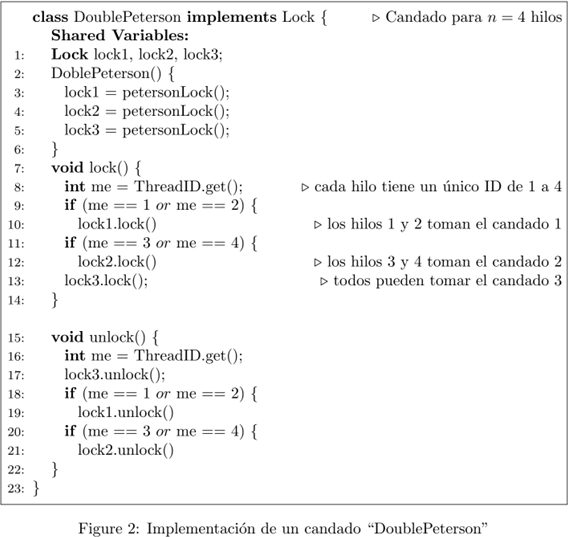
\includegraphics[width = 12 cm]{images/Figure2_tarea2.png}
    \end{center}
    
\end{enumerate}
